\chapter{Transitions-Phase Stand Heute zu Microservices}
\section{Git}
\label{chap:tranition-git}
Die \acrshort{hftm} stellte dem Betreuer in einem eigenen Git-Repository den Sourcecode bereit. Diesen habe ich anschliessend als Zip-Datei via E-Mail erhalten. Während dieser Arbeit (am 16. April) habe ich lesenden Zugriff auf das Git-Repository der \acrshort{hftm} erhalten \cite{gitlab.com/solidus/hefei}. 

\subsection{Ist-Zustand}
Beim Betrachten des eingecheckten Codes ist aufgefallen, dass beide Code-Repos Projekt-Files der \acrshort{ide} beinhalten. Teils zeigen bei solchen Daten Pfade gegen das User-Home des Commiters. Auch sind Log-Dateien und Libraries / Abhängigkeiten (lib / Jar-Files) im Git des Projekts eingecheckt (siehe Listing \ref{lst:gitlab-listing}). 
\begin{lstlisting}[caption={Listing der Daten im Git-Repository 'gitlab.com/solidus/hefei'},language=Bash, columns=fixed,label={lst:gitlab-listing}]
$ du -sch .[!.]* *
17M	.git
4.0K	.gitignore
4.0K	build.xml
24K	config
17M	lib
107M	logs
4.0K	manifest.mf
100K	nbCodeConvJava.zip
152K	nbproject
4.0K	README.md
3.1M	src
-------------
143M	total
\end{lstlisting}
\subsection{Soll-Zustand}
Auf den \verb|lib|-Ordner kann komplett verzichtet werden, sobald Dependencies über Maven verwaltet werden (siehe Kapitel \ref{chap:voraussetzungen} und \ref{chap:maven}). Libraries werden nicht erneut als binäres Jar-File ins Git/\acrshort{vcs}\footnote{Version Control System} hochgeladen. Der Sourcecode einer Library bleibt ebenfalls nur im \acrshort{vcs} der jeweiligen Entwickler.

Die Ordner \ctexttt{logs} und \ctexttt{nbproject} können einfach in der \ctexttt{.gitignore}-Datei auf die Blacklist gesetzt werden. Logs gehören grundsätzlich nicht ins \acrshort{vcs} und die \acrshort{ide}-spezifischen Daten werden über Maven oder die Entwicklungsumgebung selbst beim Öffnen des Projekts automatisch erstellt. Das Projekt kann vollständig in Maven definiert werden (Bsp. die Main-Klassen, Compiler-Version).

\subsection{Git Commit Message Guidelines}
Die Git Commit Nachrichten (\url{https://gitlab.com/solidus/hefei/}) halten sich nicht an die ,,Commit Guidelines'' von \href{https://git-scm.com/book/en/v2/Distributed-Git-Contributing-to-a-Project}{git-scm.com} \cite{git-scm.com-guide}. Die Commit Message sollte nach folgender Vorlage aufgebaut sein:
\begin{quote}
\begin{lstlisting}[language=none,caption={Template einer Git commit message}]
Short (50 chars or less) summary of changes

More detailed explanatory text, if necessary.  Wrap it to
about 72 characters or so.  In some contexts, the first
line is treated as the subject of an email and the rest of
the text as the body.  The blank line separating the
summary from the body is critical (unless you omit the body
entirely); tools like rebase can get confused if you run
the two together.

Further paragraphs come after blank lines.

  - Bullet points are okay, too

  - Typically a hyphen or asterisk is used for the bullet,
    preceded by a single space, with blank lines in
    between, but conventions vary here

\end{lstlisting}
\end{quote}
Die erste Zeile mit Richtwert 50 Zeichen ist die, die auf Gitlab.com und im Git CLI als Zusammenfassung auftaucht. Die History mit dem CLI-Befehl \ctexttt{git log --oneline} sieht an vielen Stellen so aus:
\begin{figure}[H]
	\centering
	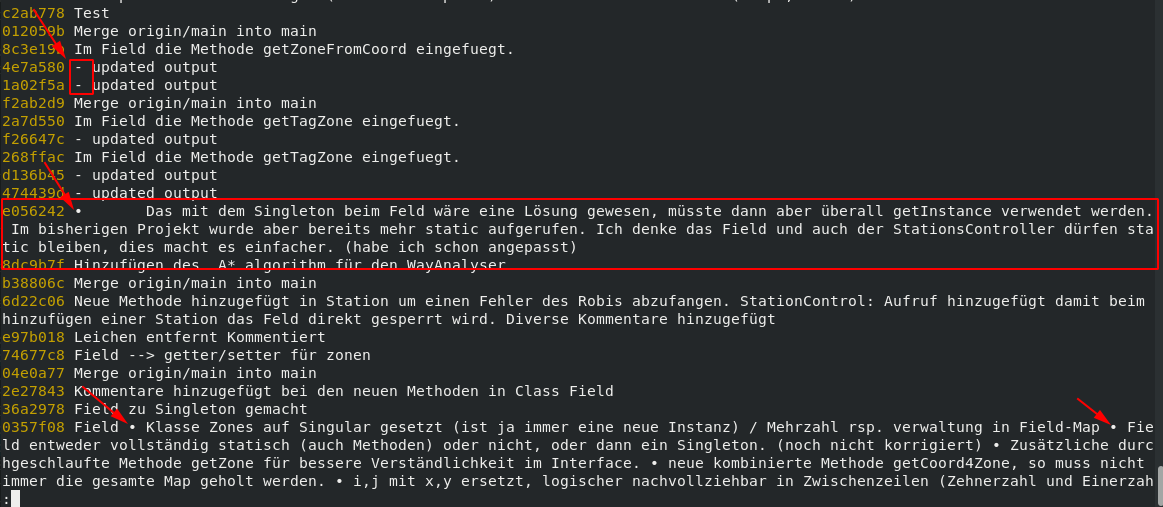
\includegraphics[width=1.0\textwidth]{img/git-commit-message.png}
	\caption{Aktuelle Git Commit History im Repository der HFTM}
	\label{fig:git-commit-message}
\end{figure}
Die Umgewöhnung ist denkbar eifach:
\begin{itemize}
	\item Erste Zeile mit einer Zusammenfassung ausfüllen (darf heute auch bisschen mehr als 50 Zeichen sein, aber nicht übertreiben)
	\item Zweite Zeile leer
	\item Alles was bisher auf der ersten Zeile geschrieben wurde, kann man jetzt ab Zeile 3 einfügen.
	\item Kein UTF-8 Aufzählungszeichen verwenden sondern das Zeichen '-' oder '*'. Fertig.
\end{itemize}

\section{Programmcode}
Beim Betrachten des Programmcodes im Gitlab-Repo der \acrshort{hftm} sind folgende Dinge aufgefallen:
\subsection{Testen der Klassen}
In sehr vielen Klassen gibt es eine Main-Methode um diese zu testen. Dabei weiss meist nur der Entwickler, was passieren soll, wenn der Code ausgeführt wird. Besser wäre hier definitiv die Umstellung auf einen Unit-Test (siehe Abschnitt \ref{sec:tests_and_unittests}). Da ist es dann für den neuen Entwickler klar: laufen die Tests erfolgreich durch, ist alles gut. Zudem kann es durch eine Build-Automatisierung automatisiert werden.

\subsection{Abkürzungen}
An vielen Stellen werden Methoden und Variablen unglücklich abgekürzt. Hier einige Beispiele:
\begin{itemize}
	\item Variable für den Java-Util-Logger heisst \ctexttt{ecm}
	\item Klasse \ctexttt{CoordCalc.java}, Methode: \ctexttt{calcCoords(IScanReflectData scanMeasData)} \\ -> Liest man den Source-Code wird es klar, die Klasse rechnet Koordinaten von polar auf kartesisch um. Also würde ich die gleich so benennen: \ctexttt{PolarToCartesian.calculate(...)}. Oder zumindest per Java-Doc dokumentieren, was die Klasse macht.
	\item Die Methode \ctexttt{calculateDistanceMMToGUIPx(int mm)} würde ich zu \ctexttt{calculateMillimeterToPixel} umbenennen.
\end{itemize}
Zusammenfassend meine Empfehlung: Klassen und Methoden nicht abkürzen vor allem wenn diese noch public sind. Sinnvolle Namen für die Variablen verwenden und diese auch nicht abkürzen.

\chapter{Korrespondenz}
\section{Mails}
\subsection{Mail zum Abkürzen der Servants}
\label{sec:servant-abkuerzern-referenz}
\begin{formal}
	\textbf{Von:} Koenig Reto\\
	\textbf{Gesendet:} Sonntag, 29. April 2018 21:41\\
	\textbf{An:} Kilchhofer Marco\\
	\textbf{Betreff:} Re: AW: AW: AW: Termin Lidar-Besprechung\\
	\\
	Hey Marco
	
	Das ganze mit dem Hin- und Her bzgl Service und Servant hat mich zum 
	Nachdenken gebracht (vielleicht nicht genug, aber ich schreib mal auf, was mir 
	in den Sinn gekommen ist)
	
	Statt dass der Intent ausschliesslich direkt Werte erhält, soll es neu möglich sein, diese Werte 'per Reference' bzw. per Subscription zu erhalten. Dabei ist zu beachten, dass die Werte, welche per Subscription erhalten werden auch in den Intent gemapped werden können.
	
	Ich hoffe Du kommst nach:
	
	Hier ein Beispiel:
	Stell Dir vor, dass der EdgeDetector Service folgenden Intent hätte:
	
	\begin{verbatim}
	Topic:
	hftm/EdgeDetector/1/I
	
	Message:
	timeStamp:<number>
	distance:[0..255]_270
	position:
	x: <number>
	y: <number>
	\end{verbatim}
	
	Nun käme neu noch die Referenz zum Intent hinzu:
	\begin{verbatim}
	Topic:
	hftm/EdgeDetector//1/I
	
	Message:
	timeStamp: <number>
	distance: [0..255]_270
	position:
	x: <number>
	y: <number>
	
	subscription: <null>
	distance: null|<String>
	position: null|<String>
	synchronization: null|<String>
	\end{verbatim}
	
	D.h.
	Entweder übergibt man eine 'distance' 'per value' oder aber man übergibt sie 'per reference', und teilt mit, wo die Daten verortet sind.
	
	Dabei ist darauf zu achten, dass die Daten am Referenzpunkt sich auf das Intent abbilden lassen müssen!
	
	Hier das LiDAR Beispiel dazu:
	Stell Dir vor, dass der LiDAR  Service folgenden Event absenden würde:
	\begin{verbatim}
	Topic:
	LiDAR/xyz/E/measurement
	
	Message:
	timeStamp: <Number>
	distance: [0..255]_270
	rssi: [0..255]_270
	\end{verbatim}
	
	Das trifft sich gut, denn wenn wir dem EdgeDetector als 'distance' die Referenz: LiDAR/xyz/E/measurement geben, dann wird der EdgeDetector bei jeder Änderung von dort eine Meldung erhalten (direkt und ohne Umweg über den Servant)
	
	Diese Meldung kann der Mapper (Jackson) auch tatsächlich in den Intent des EdgeDetectors mappen, da die 'distance' Werte dem Format entsprechen. Die 'RSSI' Werte würden in diesem Beispiel vom Mapper einfach ignoriert. (Das funktioniert bereits jetzt so)
	
	Nun wäre der EdgeDetector im Besitz eines Intents, welcher die 'distance' Werte hätte... und einen 'timeStamp'
	
	Nehmen wir weiter an, es gäbe einen PositionService, der die aktuelle Position ausgibt:
	\begin{verbatim}
	Topic:
	hftm/Positioning/1/E/position
	
	Message:
	timeStamp: <number>
	position:
	x: <number>
	y: <number>
	\end{verbatim}
	
	Wir würden dem EdgeDetector als 'position' die Referenz: hftm/Positioning/1/E/ position übergeben. Sobald sich dort also eine Änderung ergibt, wäre der EdgeDetector im Besitz eines weiteren Intents, welcher die 'position' Werte hätte... und einen 'timeStamp'
	
	Wenn der EdgeDetectorService nun beide Intents (intern) fusioniert ergibt sich ein Intent mit 'distance' und 'position' Werten. (Der 'timeStamp' würde wohl halt einfach von einem der beiden genommen)
	
	Dieser Intent wäre nun valide und könnte weiter verarbeitet werden...
	
	
	Das erzeugt ein paar Probleme, welche aber pro Service abgehandelt werden könnten:
	
	\textbf{Was geschieht, wenn danach weitere 'distance' Werte kämen, aber keine neue Position?}\\
	-> Es könnte einfach die letzte Position genommen werden und diese fusioniert werden.
	
	\textbf{Was geschieht, wenn danach weitere 'position' Werte kämen, aber keine neuen 'distance' Werte?}\\
	Das wäre bestimmt falsch, denn beim Ändern der Position würden zwingend auch die 'distance' Werte ändern... Das LiDAR scheint einfach zu 'langsam' zu sein.\\
	-> Wir teilen im Intent des EdgeDetectors mit, dass wir als 'synchronization' das Topic: 'LiDAR/xyz/E/measurement' nehmen. Also erst wenn von dort ein neuer Wert kommt, soll intern ein neuer Intent zusammengesetzt werden.
	
	\textbf{Was geschieht, wenn ein Event statt einer Message... mehrere Messages hat, also die Position zu verschiedenen Zeiten, bzw. die Distanzen zu verschiedenen Zeiten in einem Array kommen?} \\
	-> Entweder wir nehmen nur das letzte, oder aber wir versuchen ein Mapping zwischen den einzelnen Messages (anhand des Timestamps) zu machen, oder wir interpolieren, ... je nach dem, was schlau erscheint für diesen Service...
	
	Was hältst Du davon?
	
	Ich hoffe Du kannst aus dem Beispiel die Idee ableiten...
	
	L.G.
	
	Reto
\end{formal}